%%
%%::::::::::::::::::::::::::::commands
% font
%\usepackage{helvet}
%\renewcommand{\familydefault}{\sfdefault}
% sectioning
%\makeatletter

\newcommand{\subpart}[1]{%
  \vspace{2\parskip}%
  \textbf{#1}%
  \hspace*{1em}%
}
\newcommand{\subsubpart}[1]{%
  \vspace{2\parskip}%
  \textit{#1}%
  \hspace*{1em}%
}
\newcommand{\subitempart}[2][$\bullet$]{%
  \vspace{2\parskip}%
  #1\hspace{1.em}\textbf{#2}\hspace{1.em}%
}
\newcommand{\subsubitempart}[2][--]{%
  \vspace{2\parskip}%
  #1\hspace{1.em}\textit{#2}\hspace{1.em}%
}
\newcommand{\note}[2][]{%
  \textit{#2}\hspace*{1em}
}
\makeatletter
\newcommand\subxsection{\@startsection{subsection}{2}{\z@}%
                                     {-3.25ex\@plus -1ex \@minus -.2ex}%
                                     {1.5ex \@plus .2ex}%
                                     {\normalfont\large\bfseries}}
\makeatother
%\makeatother
% miscellaneous
\newenvironment{inframe}{%
\noindent
\begin{lrbox}{\setbox1}
\begin{minipage}{\linewidth}%
}{%
\end{minipage}
\end{lrbox}
\framebox{\usebox{\box1}}
}
% foot note with choice of symbol 
\long\def\symbolfootnote[#1]#2{\begingroup%
\def\thefootnote{\fnsymbol{footnote}}\footnote[#1]{#2}\endgroup}
\long\def\symbolfootnotetext[#1]#2{\begingroup%
\def\thefootnote{\fnsymbol{footnote}}\footnotetext[#1]{#2}\endgroup}
% convenience
\newcommand{\ger}[1]{\emph{#1}}
\newcommand{\lat}[1]{#1}
\newcommand{\ie}{i.e.\@}
\newcommand{\cf}{cf.\@}
\newcommand{\eg}{e.g.\@}
\newcommand{\etal}{et al.\@}
\newcommand{\intro}[1]{\emph{#1}}
\newcommand{\fail}[1]{\emph{#1}}
%\newcommand{\tc}[1]{\ovalfbox{\textsf{#1}}}
\newcommand{\tc}[1]{%
\ifmmode
  \mathchoice{
    \ovalfbox{\textsf{\text{$#1$}}}
  }{
    \ovalfbox{\textsf{\text{$#1$}}}
  }{
    \ovalfbox{\textsf{\text{$\scriptstyle #1$}}}
  }{
    \ovalfbox{\textsf{\text{$\scriptscriptstyle #1$}}}
  }
\else
\ovalfbox{\textsf{#1}}%
\fi}
\newcommand{\name}[1]{#1}
% rotate
\newcommand{\textrotl}[1]{%
\setbox2=\hbox{#1}
\rotl2
}
% source code style
\newcommand{\cod}[1]{\texttt{\textup{#1}}}
\newenvironment{codenv}{\begin{quote} \tt}{\end{quote}}
\newcommand{\cor}{$|$}
\newcommand{\cgb}{$($}
\newcommand{\cge}{$)$}
\newcommand{\ccb}{$[$}
\newcommand{\cce}{$]$}
\newcommand{\cnl}{} %%$\setminus$}
\newcommand{\chs}{\hspace{3em}}


% bold Figure 7.5 at figures
\makeatletter
\long\def\@makecaption#1#2{%
  \vskip-0.65\abovecaptionskip
  \sbox\@tempboxa{\textbf{#1:} #2}%
  \ifdim \wd\@tempboxa >\hsize
    \textbf{#1:} #2\par
  \else
    \global \@minipagefalse
    \hb@xt@\hsize{\hfil\box\@tempboxa\hfil}%
  \fi
  \vskip\belowcaptionskip}
\makeatother
%%% Local Variables: 
%%% mode: latex
%%% TeX-master: "inventory"
%%% End: 

%% mathematical abbreviations
%%\usepackage{helvet}
%%\renewcommand{\familydefault}{\sfdefault}
%\usepackage{amsmath,amssymb,color}  % and more

% extra colourful stuff
%%\newcommand{\mathbl}[1]{\text{\textcolor[rgb]{0.0,0.0,0.69}{$#1$}}}
%\newcommand{\mathbl}[1]{#1}
%%\newcommand{\mathgr}[1]{\text{\textcolor[rgb]{0.0,0.69,0.0}{$#1$}}}
%\newcommand{\mathgr}[1]{#1}

%% mathematical operators
\newcommand{\ii}{\mathrm{i}}  % complex i
\newcommand{\dd}{\mathrm{d}}  % differential d
\newcommand{\pd}{\partial}  % partial differentiation d
\newcommand{\DD}{\mathrm{D}}  % linearisation operator
\newcommand{\Alpha}{\mathcal{A}}
\newcommand{\levicivita}{\mathcal{E}}  % Levi-Civita symbol
%\newcommand{\tns}[1]{\underline{\boldsymbol{#1}}}  % tensor
%\newcommand{\tnsfour}[1]{\mathsf{#1}}
\newcommand{\tns}[2][0]{
\def\myinput{#2}
% \count0=#1
% \ifnum\count0=1
%   \def\myinput{#2}
% \fi
% \ifnum\count0=2
%   \def\myinput{#2}
% \fi
% \ifnum\count0=4
%   \def\myinput{\tnsfour{#2}}
% \fi
\dimen1=0.5pt  % truncation length of underline
\mathchoice{
  \setbox0=\hbox{$\boldsymbol{\myinput{}}$}
  \dimen2=\wd0
  \ifdim\dimen2>\dimen1
    \advance\dimen2 by -2\dimen1
  \fi
  \wd0=\dimen2
  \setbox1=\hbox{\hskip\dimen1\underline{\hskip-\dimen1\box0}\hskip2\dimen1}
  \box1
}{
  \setbox0=\hbox{$\boldsymbol{\textstyle \myinput{}}$}
  \dimen2=\wd0
  \ifdim\dimen2>\dimen1
   \advance\dimen2 by -2\dimen1
  \fi
  \wd0=\dimen2
  \setbox1=\hbox{\hskip\dimen1\underline{\hskip-\dimen1\box0}\hskip2\dimen1}
  \box1
}{
  \setbox0=\hbox{$\boldsymbol{\scriptstyle \myinput{}}$}
  \dimen2=\wd0
  \ifdim\dimen2>\dimen1
    \advance\dimen2 by -2\dimen1
  \fi
  \wd0=\dimen2
  \setbox1=\hbox{\hskip\dimen1\underline{\hskip-\dimen1\box0}\hskip2\dimen1}
  \box1
}{
  \setbox0=\hbox{$\boldsymbol{\scriptscriptstyle \myinput{}}$}
  \dimen2=\wd0
  \ifdim\dimen2>\dimen1
    \advance\dimen2 by -2\dimen1
  \fi
  \wd0=\dimen2
  \setbox1=\hbox{\hskip\dimen1\underline{\hskip-\dimen1\box0}\hskip2\dimen1}
  \box1
}}
\newcommand{\hattns}[1]{\hat{\tns{#1}}}  % tensor with hat
\newcommand{\dottns}[1]{\dot{\tns{#1}}}  % tensor with dot
\newcommand{\bartns}[1]{\bar{\tns{#1}}}  % tensor with bar
\newcommand{\bretns}[1]{\breve{\tns{#1}}}  % tensor with breve
\newcommand{\chetns}[1]{\check{\tns{#1}}}  % tensor with check
\newcommand{\tiltns}[1]{\tilde{\tns{#1}}}  % tensor with tilde
\newcommand{\ddottns}[1]{\ddot{\tns{#1}}}  % tensor with to dots
\newcommand{\mat}[1]{\boldsymbol{#1}}  % matrix
\newcommand{\barmat}[1]{\bar{\mat{#1}}}  % matrix with bar
\newcommand{\vct}[1]{\boldsymbol{#1}}  % vector
\newcommand{\hatvct}[1]{\hat{\vct{#1}}}  % vector with hat
\newcommand{\hatdotvct}[1]{\hat{\dotvct{#1}}}  % vector with hat and dot
\newcommand{\dotvct}[1]{\dot{\vct{#1}}}  % vector with dot
\newcommand{\ddotvct}[1]{\ddot{\vct{#1}}}  % vector with double dots
\newcommand{\dddotvct}[1]{\dddot{\vct{#1}}}  % vector with triple dots
\newcommand{\barvct}[1]{\bar{\vct{#1}}}  % vector with bar
\newcommand{\tildevct}[1]{\tilde{\vct{#1}}}  % vector with tilde
\newcommand{\tilvct}[1]{\tilde{\vct{#1}}}  % vector with tilde
\newcommand{\chevct}[1]{\check{\vct{#1}}}  % vector with check
\newcommand{\T}{\mathrm{T}}  % transpose T
\newcommand{\bre}[1]{\breve{#1}}  % short for breve
\newcommand{\che}[1]{\check{#1}}  % short for check
\newcommand{\adiag}[1]{\overset{\scriptscriptstyle\smallsetminus}{#1}}
\newcommand{\alowtri}[1]{\overset{\scriptscriptstyle\llcorner}{#1}}
\newcommand{\grad}{\mathrm{grad}}  % (spatial) gradient
\newcommand{\Grad}{\mathrm{Grad}}  % (material) gradient
\newcommand{\ddiv}{\mathrm{div}}  % divergence in spatial frame
\newcommand{\Ddiv}{\mathrm{Div}}  % divergence in material frame
\newcommand{\dirac}{\delta}  % Dirac's delta
\newcommand{\cof}{\mathrm{cof}}  % (spatial) gradient
\newcommand{\forwhich}{\;|\;}
% \newcommand{\ass}[3][d]{%  % assembly operator, 'd' display style, 't' text style
% \if#1d
% \overset{#3}{\underset{#2}{\raisebox{-0.6ex}{\mbox{\huge $\mathsf{A}$}}}}
% \else
% \raisebox{-0.4ex}{\mbox{\Large $\mathsf{A}$}}_{#2}^{#3}
% \fi
% }
\newcommand{\Ass}[3][d]{%  % assembly operator
% option 'd' is useless
\mathchoice{  % display style
\overset{#3}{\underset{#2}{\raisebox{-0.6ex}{\mbox{\huge $\mathsf{A}$}}}}
}{  % text style
\raisebox{-0.35ex}{\mbox{\Large $\mathsf{A}$}}_{#2}^{#3}
}{  % script style
\raisebox{-0.35ex}{\mbox{\Large $\mathsf{A}$}}_{#2}^{#3}
}{  % scriptscript style
\raisebox{-0.35ex}{\mbox{\Large $\mathsf{A}$}}_{#2}^{#3}
}}

\newcommand{\loc}{\mathrm{loc}}  % location mapping
\newcommand{\stat}{\mathrm{stat}}  % location mapping
\newcommand{\domainsum}{\bigcup}
\newcommand{\abs}[1]{|#1|}
\newcommand{\Abs}[1]{\|#1\|}
% \ifmmode ... \else ... \fi
\newcommand{\Nabla}{\nabla_{\!0}}
\newcommand{\incr}{\Delta}
\newcommand{\Lin}{\mathrm{Lin}}  % linearisation
\newcommand{\trace}{\mathrm{tr}}  % trace of quadratic tensor

%% symbols
\newcommand{\eps}{\varepsilon}  % epsilon
\newcommand{\sig}{\sigma}  % epsilon
\newcommand{\const}{\mathrm{const}}  % constant
\newcommand{\R}{\mathbb{R}}  % real set of numbers R
\newcommand{\CC}{\mathbb{C}}  % complex set of numbers C
\newcommand{\ndof}{\mathit{ndof}}  % number of degrees of freedom
\newcommand{\nnod}{\mathit{nnod}}  % number of nodes
\newcommand{\nele}{\mathit{nele}}  % number of elements
\newcommand{\eenh}{\mathit{eenh}}  % number of element enhancements
\newcommand{\enod}{\mathit{enod}}  % number of element nodes
\newcommand{\numgp}{\mathit{numgp}}  % number of Gausspoints in direction 
\newcommand{\nco}{\mathit{nco}}  % number of active contact sets 
\newcommand{\BE}{\text{BE}}  % balance equations
\newcommand{\FBC}{\text{FBC}}  % flux boundary conditions
\newcommand{\DBC}{\text{DBC}}  % Dirichlet boundary conditions
\newcommand{\TPE}{\text{TPE}}  % total potential energy
\newcommand{\EEE}{\text{EE}}  % strain-strain connection
\newcommand{\SSS}{\text{SS}}  % stress-stress connection
\newcommand{\FFF}{\text{FF}}  % defgrad-defgard connection
\newcommand{\PPP}{\text{PP}}  % 1PK-1PK stress connection 
\newcommand{\HR}{\text{HR}}  % Hellinger--Reissner
\newcommand{\HW}{\text{HW}}  % Hu--Washizu
\newcommand{\Int}{\text{int}}  % internal
\newcommand{\Ext}{\text{ext}}  % external
\newcommand{\HOT}{\mathit{HOT}}  % higher order terms
\newcommand{\Dt}{\Delta t}  % time step size
\newcommand{\effdyn}{\text{effdyn}}  % effective dynamic
\newcommand{\Teffdyn}{\text{Teffdyn}}  % effective dynamic
\newcommand{\PK}{\text{PK2}}  % 2nd Piola--Kirchhoff
\newcommand{\Pk}{\text{PK1}}  % 1st Piola--Kirchhoff
\newcommand{\KI}{\text{K}}  % Kirchhoff
\newcommand{\GL}{\text{GL}}  % Green--Lagrange
\newcommand{\EA}{\text{E}}  % Euler--Almansi
\newcommand{\Eng}{\text{i}}  % engineering
\newcommand{\Nat}{\text{n}}  % natural / logarithmic
\newcommand{\TSO}{\textrm{II}}  % theory of second order
\newcommand{\TFO}{\textrm{I}} % theory of 1st order
\newcommand{\CT}{\text{C}}  % Cauchy / true
\newcommand{\BI}{\text{B}}  % Biot
\newcommand{\VK}{\text{VK}}  % St. Venant-Kirchhoff
\newcommand{\Tang}{\text{T}}  % tangential
\newcommand{\ela}{\text{e}}  % elastic
\newcommand{\geo}{\text{g}}  % geometric
\newcommand{\ini}{\text{u}}  % initial
\newcommand{\loa}{\text{L}}  % load
\newcommand{\tol}{\mathit{tol}}  % tolerance
\newcommand{\LL}{\text{L}}  % `linear'
\newcommand{\enh}{\mathit{enh}}  % enhanced
\newcommand{\red}{\text{red}}  % reduced
\newcommand{\crit}{\text{crit}}  % critical
\newcommand{\Inva}{I}
\newcommand{\INva}{I\!\!I}
\newcommand{\INVa}{I\!\!I\!\!I}
\newcommand{\Mat}{\text{m}}


%% convenience
\newcommand{\unit}[1]{\,\mathrm{#1}}  % unit
\newcommand{\EE}[1]{\cdot 10^{#1}}  % "scientific notation" for 10 to the power of 
\newcommand{\virt}{\delta}  % variation of first kind / virtual
\newcommand{\set}[1]{\mathcal{#1}}  % set
\newcommand{\script}[1]{\mathcal{#1}}

%% text font stuff
\newcommand{\period}{\text{.}}
\newcommand{\comma}{\text{,}}
%\newcommand{\colon}{\text{:}}
\newcommand{\semicolon}{\text{;}}

%% circled text (EgyptTeX)
%%\newcommand{\tc}[1]{%
%%\ifmmode
%%  \mathchoice{
%%    \ovalfbox{\textsf{\text{$#1$}}}
%%  }{
%%    \ovalfbox{\textsf{\text{$#1$}}}
%%  }{
%%    \ovalfbox{\textsf{\text{$\scriptstyle #1$}}}
%%  }{
%%    \ovalfbox{\textsf{\text{$\scriptscriptstyle #1$}}}
%%  }
%%\else
%%\ovalfbox{\textsf{#1}}%
%%\fi}

%% special
\newcommand{\sboxed}[1]{\boxed{\scriptstyle#1}}
\newcommand{\Underline}[1]{\underline{\underline{#1}}}  % double underline
\newcommand{\underneath}[3][0pt]{  % place text underneath symbol
\setbox0=\hbox{$|$}
\dimen2=\ht0
\advance\dimen2 by #1
\setbox0=\hbox{\vrule height\dimen2}
\setbox1=\hbox{$\displaystyle #2$}
\setbox5=\hbox{$#3$}
\dimen5=\dp5
\advance\dimen5 by 2pt
\setbox2=\hbox{\vrule width0pt height\ht5 depth\dimen5 \box5}
\dimen0=\dp0
\advance\dimen0 by \ht2
\advance\dimen0 by 2pt
\dimen1=0.5\wd1
\ifdim\wd1>\wd2
\dimen4=0.5\wd2
\else
\dimen4=0.5\wd1
\fi
\setbox3=\hbox{\copy0\hskip-\dimen4\lower\dimen0\copy2}
\dimen3=\ht3
\advance\dimen3 by \dp1
\advance\dimen3 by 2pt
\setbox4=\hbox to \wd1 {\copy1\hskip-\dimen1\lower\dimen3\copy3}
\box4
}
\newcommand{\overneath}[3][0pt]{  % place text underneath symbol
\setbox0=\hbox{$|$}
\dimen2=\ht0
\advance\dimen2 by #1
\setbox0=\hbox{\vrule height\dimen2}
\setbox1=\hbox{$\displaystyle #2$}
\setbox2=\hbox{$#3$}
\dimen0=\ht0
\advance\dimen0 by \dp2
\advance\dimen0 by 2pt
\dimen1=0.5\wd1
\ifdim\wd1>\wd2
\dimen4=0.5\wd2
\else
\dimen4=0.5\wd1
\fi
\setbox3=\hbox{\copy0\hskip-\dimen4\raise\dimen0\copy2}
\dimen3=\ht1
%\advance\dimen3 by \ht1
\advance\dimen3 by 2pt
\setbox4=\hbox to \wd1 {\copy1\hskip-\dimen1\raise\dimen3\copy3}
\box4
}
%%
%%
\makeatletter
\newcommand{\strikethrough}[2][d]{%
\unitlength=1pt%
\newcount\extraspace
\extraspace=5
\newbox\arg%
% switch to (displayed) math mode
\ifmmode  % switch to (displayed) math mode or text mode
\if#1d  % switch to display style if 'd' option
\setbox\arg=\hbox{$\displaystyle #2$}%
\else  % switch to text style  if 't' option
\setbox\arg=\hbox{$\textstyle #2$}%
\fi
\else
\setbox\arg=\hbox{#2}%
\fi
% get argdepth
\newcount\argdepth%
\setbox1=\hbox{%
\global\argdepth=\strip@pt\dp\arg
\global\advance\argdepth by \the\extraspace
}%
% get argheight
\newcount\argheight%
\setbox1=\hbox{%
\global\argheight=\strip@pt\ht\arg
\global\advance \argheight by \the\argdepth
%\global\advance \argheight by \the\extraspace
}%
% get argwidth
\newcount\argwidth%
\setbox1=\hbox{%
\global\argwidth=\strip@pt\wd\arg
\global\advance\argwidth by \the\extraspace
\global\advance\argwidth by \the\extraspace
}%
% create output box
\newbox\product%
\setbox\product=\hbox{%
\begin{picture}(\the\argwidth,\the\argheight)
% draw a nice box (debug purposes)
%\put(0,-\the\argdepth){\line(1,0){\the\argwidth}}
%\put(0,-\the\argdepth){\line(0,1){\the\argheight}}
%\put(0,-\the\argdepth){\line(0,1){\the\argheight}}
%\put(0,\strip@pt\ht\arg){\line(1,0){\the\argwidth}}
\qbezier(0,-\the\argdepth)(0,-\the\argdepth)(\the\argwidth,\the\argheight)
%\put(\the\argwidth,\the\argheight){tip}  % debug purposes
\put(\the\extraspace,0){\box\arg}
\end{picture}}%
\box\product%
}
\makeatother

%%% Local Variables: 
%%% mode: plain-tex
%%% TeX-master: "fe"
%%% End: 



%%
%%----------------------------materials
\chapter{Materials}

\section{How to add a material to CCADISCRET}
Here it's briefly described as a step-by-step guide how to add a material to the new discretization of baci. Please look at already implemented materials to get a better idea of what to do.

\begin{itemize}
 \item Choose appropriate names for your material model and add new files \textit{$<$material name$>$.cpp} and \textit{$<$material name$>$.H} to the folder \textit{src/drt\_mat/}. Define the necessary object best by looking at other materials.

\item Add a case definiton to the top of \textit{src/drt\_mat/material.cpp} accordingly to other materials there:
\begin{verbatim}
  case m_<material name>:
    return Teuchos::rcp(new <material name>(actmat));
\end{verbatim}

\item Define the unique parobject number in \textit{src/drt\_lib/drt\_parobject.H.cpp}:
\begin{verbatim}
 #define ParObject_<material name>               (int)<next available number>
\end{verbatim}

\item Add the material structure (all input parameters for the material) to \textit{src/headers/materials.h} to the global materials structure \textit{\_MATERIALS} 
\begin{verbatim}
 struct _<material name>          *<material name>;       /* comments are always welcome */
\end{verbatim}
and subsequently to the complete structure beneath it:
\begin{verbatim}
typedef struct _<material name>
{
     double	   density;
} <material name>;
\end{verbatim}

\item Add your material name to the \textit{enum \_MATERIAL\_TYP} structure at \textit{src/headers/enums.h}:
\begin{verbatim}
 m_<material name>        /* coments are really welcome */
\end{verbatim}

\item Get your material read from the input file at \textit{src/drt\_lib/input\_material\_ccadiscret.cpp} by adding a read block:
\begin{verbatim}
frchk("<material name in input file>",&ierr);
if (ierr==1)
{
   localmat.mattyp = m_<material name>;
   localmat.m.<material name> = new <material name>();
   frdouble("DENS",&(localmat.m.<material name>->density)        ,&ierr);
}
\end{verbatim}

\item Add the parobject for the postprocessing at \textit{src/drt\_lib/drt\_utils.cpp}
\begin{verbatim}
case ParObject_BioCell:
{
   MAT::<material name>* material = new MAT::<material name>();
   material->Unpack(data);
   return material;
}
\end{verbatim}

\item Finally let baci know that it should compile the new files at \textit{OBJS\_DRT\_MAT\_LIB} in the file \textit{Makefile.objects}. Add the objectfile to the list:
\begin{verbatim}
src/drt_mat/<material name>.o \
\end{verbatim}

\item Now it's still necessary to let your element know, that it can use the material. For e.g. the solid 3 you would need to change \textit{src/drt\_so3/so\_material.cpp}.
\begin{verbatim}
case m_<material name>: /*----------------- comments are so useful */
{
   MAT::<material name>* material = static_cast <MAT::<material name>*>(mat.get());
   material->Evaluate(glstrain,cmat,stress);
   *density = material->Density();
   break;
}
\end{verbatim}

\end{itemize}

Reconfigure and compile baci and your material should be fine and running (in case its linear elastic ;-).


\section{Global Materials}

Some old email
\begin{verbatim}
-------- Original Message --------
Subject: Re: ccarat materials
Date: Tue, 07 Mar 2006 12:42:01 +0100
From: Stefan Hartmann <hartmann@statik.uni-stuttgart.de>
To: Burkhard Bornemann <bornemann@lnm.mw.tum.de>

Hallo Brukhard,
gschichtlich ist es so, dass jedes Element seine eigenen 
Materialroutinen hat. Als ich hier angefangen habe, hat es aber so ein 
bisschen geheissen, dass es evtl. ganz schoen weare, wenn die 
Materialgeschichten vom Element entkoppelt sind. Daraufhin habe ich 
diejenigen Sachen, die ich neu programmiert habe so geschrieben, dass 
sie allgemein 3D-Formuliert sind. D.h. diese Routinen sind dann mit ein 
paar entsprechenden Koordinatentransformationen fuer das Shell8/9 und 
Brick1 verwendbar. Fuer das Wall habe ich entsprechende Huellroutinen 
geschrieben, die die plane-strain/stress Geschichte in den Griff bekommt 
und die notwendige Kondensation der Werkstoffmatrix durchfuehrt.
[...]
Gruss,
Stefan

Burkhard Bornemann wrote:

> Hallo Stefan,
>
> ich versuche gerade einen Ueberblick ueber die Stellen in Ccarat zu 
> bekommen, an denen die Materialien fuer die Strukturen definiert 
> werden. Mir ist aufgefallen, dass der Ordner src/materials nur (?) von 
> Wall1 und Shell9 verwendet wird. Die anderen Strukturelemente haben 
> separate Materialdefs (oder?).
>
> Ist es geplant alle Materialen ueber src/materials gemeinsam zu 
> definieren, oder gar das Gegenteil? Ueber einen kleinen Tipp, waere 
> ich echt froh.
>
> wall1 & shell9 ==> Definitionen im materials/* Ordner
> brick1 ==> eigene Materialdefinitionen
> shell8 ==> eigene Materialdefinitionen
> beam3 ==> eigene Materialdefinitionen
>
>
> Beste Gruesse
> Burkhard
>
\end{verbatim}

Routines for global materials are located in src/materials.\\
`\cnl' is for line continuation.


\subsection{St. Venant Kirchhoff}

\cod{MAT\_Struct\_StVenantKirchhoff} \\ \\
\textbf{input:}  
\begin{quote}
\begin{tabular}{ll}
\cod{MAT} $int$ \cnl & \\
\cod{YOUNG} $real$ \cnl & Young's modulus \\
\cod{NUE} $real$ \cnl & Poisson's ratio $\nu\in[0,0.5)$\\
\cod{DENS} $real$ \cnl& density $>0$\\
\cod{THEXPANS} $real$ & thermal expansion coefficient
\end{tabular} \\ \\
\end{quote}
\textbf{example:}\\ 
\cod{MAT} 1 \cod{MAT\_Struct\_StVenantKirchhoff} \cod{YOUNG} 1000.0 \cod{NUE} 
0.3 \cod{DENS} 0.001 \cod{THEXPANS} 0.0078\\ \\
\textbf{comment:}\\ 
Currently called by no elemental material routine.


\subsection{Linear elastic orthotropic material}

\cod{MAT\_Struct\_Orthotropic} \\ \\
\textbf{input:} 
\begin{quote}
\begin{tabular}{ll}
\cod{MAT} $int$ \cnl & \\
\cod{EMOD1} $real$ \cnl& Young's modulus \\
\cod{EMOD2} $real$ \cnl& Young's modulus \\
\cod{EMOD3} $real$ \cnl& Young's modulus \\
\cod{GMOD12} $real$ \cnl& shear modulus \\
\cod{GMOD13} $real$ \cnl& shear modulus \\
\cod{GMOD23} $real$ \cnl& shear modulus \\
\cod{XNUE12} $real$ & Poisson's ratio $\nu\in[0,0.5)$\\
\cod{XNUE13} $real$ \cnl& Poisson's ratio $\nu\in[0,0.5)$\\
\cod{XNUE23} $real$ & Poisson's ratio $\nu\in[0,0.5)$
\end{tabular} \\ \\
\end{quote}
\textbf{example:}\\ 
\cod{MULTIMAT} 1 \cod{MAT\_Struct\_Orthotropic} \cod{EMOD1} 31100 \cod{EMOD2} 
7600 \cod{EMOD3} 7600 \cod{GMOD12} 2900 \cod{GMOD13} 2900 \cod{GMOD23} 2600 
\cod{XNUE12} 0.303 \cod{XNUE13} 0.303 \cod{XNUE23} 0.303\\ \\
\textbf{testfile:}\\
Input/shell9\_kreuz\_easnl.dat\\ \\
\textbf{comment:}\\ 
Called by shell9.

\newpage
\subsection{Drucker-Prager material law}

\cod{MAT\_DP\_Plastic} \\ \\
\textbf{input:} 
\begin{quote}
\begin{tabular}{ll}
\cod{MAT} $int$ \cnl & \\
\cod{YOUNG} $real$ \cnl& Young's modulus \\
\cod{NUE} $real$ \cnl& Poisson's ratio $\nu\in[0,0.5)$\\
(\cod{ALFAT} $real$ \cnl& temperature expansion factor)\\
\cod{Sigy} $real$ \cnl& yield stress \\
\cod{PHI} $real$ \cnl& angle of friction\\
\cod{Hard} $real$ \cnl& Hardening modulus (if hardening) \\
\cod{GF} $real$ \cnl& fracture energy (if softening)  \\
\cod{BETAH} $real$ & controls the isotropic/kinematic hardening
\end{tabular} \\ \\
\end{quote}
\textbf{example:}\\ 
\cod{MULTIMAT} 1 \cod{MAT\_DP\_Plastic} \cod{YOUNG} 30e3 \cod{NUE} 0.0 \cod{Sigy} 
2.0 \cod{BETAH} 0.0 \cod{Hard} -0.3 \cod{PHI} 40.0 \\ \\
\textbf{testfiles:}\\
Input/shell9\_dpmisGF.dat\\
Input/shell9\_matnl.dat \\ \\
\textbf{comment:}\\ 
\cod{ALFAT} can be read in (in src/input\_full/input\_material.c) but is not used.\\
Called by shell9.


\subsection{Elastoplastic concrete material 3D}

\label{global_concrete}
\cod{MAT\_3DConcretePlastic} \\ \\
\textbf{input:} 
\begin{quote}
\begin{tabular}{ll}
\cod{MAT} $int$ \cnl & \\
\cod{YOUNG} $real$ \cnl& Young's modulus \\
\cod{NUE} $real$ \cnl& Poisson's ratio $\nu\in[0,0.5)$\\
\cod{FTM} $real$ \cnl& tensile strength \\
\cod{FCM} $real$ \cnl& compressive strength \\
\cod{GT} $real$ \cnl& tensile fracture energy \\
\cod{GC} $real$ \cnl& compressive fracture energy \\
(\cod{DFAC} $real$ \cnl& damage factor: $0.0$ plastic - $1.0$ fully damaged)\\
\cod{GAMMA1} $real$ \cnl& fitting parameter yield function 1\\
\cod{GAMMA2} $real$ \cnl& symm. biaxial compression stressfactor\\
\cod{GAMMA3} $real$ \cnl& fitting parameter to account for HPC \\
&$\to$ Haufe ($=\frac{1}{3}$ for normal concrete)\\
\cod{GAMMA4} & fitting parameter to account for HPC \\
&$\to$ Haufe ($=\frac{4}{3}$ for normal concrete)
\end{tabular} \\ \\
\end{quote}
\textbf{example:}\\ 
\cod{MAT} 1 \cod{MAT\_3DConcretePlastic} \cod{YOUNG} 30000.0 \cod{NUE} 0.2 
\cod{FTM} 3.0 \cod{FCM} 40.0 \cod{GT} 0.12 \cod{GC} 50.0 \\ \\
\textbf{testfiles:}\\ 
Input/w1\_epc3D.dat \\ 
Input/shell9\_epc.dat \\ \\
\textbf{comment:}\\ 
Only concrete, no rebars.\\
See thesis of Menrath and Haufe.\\
An unsymmetric solver should be used if trial stresses could be in the apex 
region (general warning print out is done).\\
Default values: \cod{DFAC}$=0.5$, \cod{GAMMA1}$=3.0$, \cod{GAMMA2}
$=\frac{6.0}{5.0}$, \cod{GAMMA3}$=\frac{1.0}{3.0}$, \cod{GAMMA4}$=\frac{4.0}{3.0}$.\\
\cod{DFAC} can be read in (in src/input\_full/input\_material.c) but is not used.\\
Called by wall1 and shell9.


\subsection{Anisotropic plasticity model based on Hoffman criterion}

\cod{MAT\_HoffPlastic} \\ \\
\textbf{input:} 
\begin{quote}
\begin{tabular}{ll}
\cod{MAT} $int$ \cnl & \\
\cod{EMOD1} $real$ \cnl& Young's modulus \\
\cod{EMOD2} $real$ \cnl& Young's modulus \\
\cod{EMOD3} $real$ \cnl& Young's modulus \\
\cod{GMOD12} $real$ \cnl& shear modulus \\
\cod{GMOD13} $real$ \cnl& shear modulus \\
\cod{GMOD23} $real$ \cnl& shear modulus \\
\cod{XNUE12} $real$ \cnl& Poisson's ratio $\nu\in[0,0.5)$\\
\cod{XNUE13} $real$ \cnl& Poisson's ratio $\nu\in[0,0.5)$\\
\cod{XNUE23} $real$ \cnl& Poisson's ratio $\nu\in[0,0.5)$\\
\cod{UNIAX} $real$\\
\textit{new line in inputfile}\\
\cod{S11T} $real$ \cnl& tensile strength in fiber direction\\
\cod{S11C} $real$ \cnl& compressive strength in fiber direction\\
\cod{S22T} $real$ \cnl& tensile strength perpendicular to fiber direction\\
\cod{S22C} $real$ \cnl& compressive strength perpendicular to fiber direction\\
\cod{S33T} $real$ \cnl& tensile strength perpendicular to fiber direction\\
\cod{S33C} $real$ \cnl& compressive strength perpendicular to fiber direction\\
\cod{S12} $real$ \cnl& shear strength\\
\cod{S23} $real$ \cnl& shear strength\\
\cod{S13} $real$ & shear strength\\
\textit{new line in inputfile}\\
\cod{SH11T} $real$ \cnl\\
\cod{SH11C} $real$ \cnl\\
\cod{SH22T} $real$ \cnl\\
\cod{SH22C} $real$ \cnl\\
\cod{SH33T} $real$ \cnl\\
\cod{SH33C} $real$ \cnl\\
\cod{SH12} $real$ \cnl\\
\cod{SH23} $real$ \cnl\\
\cod{SH13} $real$ \\
\textit{new line in inputfile}\\
\cod{HA11T} $real$ \cnl\\
\cod{HA11C} $real$ \cnl\\
\cod{HA22T} $real$ \cnl\\
\cod{HA22C} $real$ \cnl\\
\cod{HA33T} $real$ \cnl\\
\cod{HA33C} $real$ \cnl\\
\cod{HA12} $real$ \cnl\\
\cod{HA23} $real$ \cnl\\
\cod{HA13} $real$
\end{tabular} \\ \\
\end{quote}
\textbf{example:}\\ 
\cod{MULTIMAT} 1 \cod{MAT\_HoffPlastic} \cod{EMOD1} 21e3 \cod{EMOD2} 21e3 \cod{EMOD3} 
21e3 \cod{GMOD12} 10.5e3 \cod{GMOD23} 10.5e3 \cod{GMOD13} 10.5e3 \cod{XNUE12} 0.0 
\cod{XNUE23} 0.0 \cod{XNUE13} 0.0 \cod{UNIAX} 4.2 \\
\cod{S11T} 4.2 \cod{S11C} 4.2 \cod{S22T} 4.2 \cod{S22C} 4.2 \cod{S33T} 4.2 \cod{S33C} 
4.2 \cod{S12} 2.4 \cod{S23} 2.4 \cod{S13} 2.4 \\
\cod{SH11T} 4.2 \cod{SH11C} 4.2 \cod{SH22T} 4.2 \cod{SH22C} 4.2 \cod{SH33T} 4.2 
\cod{SH33C} 4.2 \cod{SH12} 2.4 \cod{SH23} 2.4 \cod{SH13} 2.4 \\
\cod{HA11T} 0.01 \cod{HA11C} 0.01 \cod{HA22T} 0.01 \cod{HA22C} 0.01 \cod{HA33T} 0.01 
\cod{HA33C} 0.01 \cod{HA12} 0.01 \cod{HA23} 0.01 \cod{HA13} 0.01\\ \\
\textbf{testfile:}\\ 
Input/shell9\_matnl.dat \\ \\
\textbf{comment:}\\ 
See thesis of Hoermann, p.57 ff.\\
Called by shell9.


\subsection{Von Mises material law 3D}

\label{global_mises}
\cod{MAT\_3DMisesPlastic} \\ \\
\textbf{input:} 
\begin{quote}
\begin{tabular}{ll}
\cod{MAT} $int$ \cnl & \\
\cod{YOUNG} $real$ \cnl& Young's modulus \\
\cod{NUE} $real$ \cnl& Poisson's ratio $\nu\in[0,0.5)$\\
\cod{Sigy} $real$ \cnl& yield stress \\
\cod{BETAH} $real$ \cnl& controls the isotropic/kinematic hardening \\
\cod{Hard} $real$ \cnl& Hardening modulus (if hardening) \\
\cod{GF} $real$ \cnl& fracture energy (if softening) \\
(\cod{ALFAT} $real$ & temperature expansion factor) \\
\end{tabular} \\ \\
\end{quote}
\textbf{example:}\\ 
\cod{MAT} 1 \cod{MAT\_3DMisesPlastic} \cod{YOUNG} 25850.0 \cod{NUE} 0.18 \cod{Sigy} 
1.9 \cod{GF} 0.06\\ \\
\textbf{testfile:}\\ 
Input/w1\_3DmisGF.dat \\ 
Input/shell9\_matnl.dat\\ \\
\textbf{comment:}\\ 
Plasticity model based on the von Mises yield criterion with a combined isotropic 
and kinematic hardening law (see Simo \& Hughes).\\
\cod{ALFAT} can be read in (in src/input\_full/input\_material.c) but is not used.\\
Called by wall1 and shell9.



\section{beam3}

Corresponding routine: b3\_call\_mat\\
`\cnl' is for line continuation.


\subsection{St. Venant Kirchhoff}

\cod{MAT\_Struct\_StVenantKirchhoff} \\ \\
\textbf{input:} 
\begin{quote}
\begin{tabular}{ll}
\cod{MAT} $int$ \cnl & \\
\cod{YOUNG} $real$\cnl& Young's modulus \\
\cod{NUE} $real$\cnl& Poisson's ratio $\nu\in[0,0.5)$\\
(\cod{DENS} $real$\cnl& density $>0$) \\
(\cod{THEXPANS $real$} & thermal expansion coefficient)
\end{tabular} \\ \\
\end{quote}
\textbf{example:}\\ 
\cod{MAT} 1 \cod{MAT\_Struct\_StVenantKirchhoff} \cod{YOUNG} 1.0 \cod{NUE} 0.0 
\cod{DENS} 0.0\\ \\
\textbf{testfile:}\\ 
Input/b3\_elast.dat \\ \\
\textbf{comment:}\\ 
Parameters in parentheses can be read in (in src/input\_full/input\_material.c) but are not used.


\subsection{Von Mises material law}

\cod{MAT\_MisesPlastic} \\ \\
\textbf{input:} 
\begin{quote}
\begin{tabular}{ll}
\cod{MAT} $int$ \cnl & \\
\cod{YOUNG} $real$ \cnl& Young's modulus \\
\cod{NUE} $real$ \cnl& Poisson's ratio $\nu\in[0,0.5)$\\
\cod{ALFAT} $real$ \cnl& temperature expansion factor \\
\cod{Sigy} $real$ \cnl& yield stress \\
(\cod{BETAH} $real$ \cnl& controls the isotropic/kinematic hardening) \\
\cod{Hard} $real$ \cnl& Hardening modulus (if hardening) \\
\cod{GF} $real$ & fracture energy (if softening) \\
\end{tabular} \\ \\
\end{quote}
\textbf{example:}\\ 
\cod{MAT} 1 \cod{MAT\_MisesPlastic} \cod{YOUNG} 21000000.0 \cod{NUE} 0.0 \cod{Xsi} 1.2 \cod{Sigy}
200000.0 \cod{Hard} 0.0 \cod{GF} 0.0 \cod{BETAH} 0.0 \\ \\
\textbf{testfile:}\\ 
Input/b3\_matnln.dat \\ \\
\textbf{comment:}\\ 
\cod{XSI} (see example) is not read in.\\
\cod{BETAH} can be read in (in src/input\_full/input\_material.c) but is not used.



\section{brick1}


\subsection{Itskov material law for soft collagenous tissues}

The function describes an inkompressibel hyperelastic material model based on the following papers:
\begin{itemize}
	\item (1) Itskov, Ehret, Mavrilas (2006) {\it A polyconvex anisotropic strain-energy function for soft colagenous tissues}
	\item (2) Ehret, Itskov (2007) {\it A polyconvex hyperelastic model for fiber-reinforced materials in application to soft tissues}
	\item (3) Balzani, Neff, Schroeder, Holzapfel (2005) {\it A Polyconvex Framework for Soft Biological Tissues. Adjustment to experimental Data.}
\end{itemize}

\subsubsection*{Strain-energy-function:}
It is described by a strain energy function given in (1) which for the inkompressible, isotropic case takes the form
\begin{displaymath}
	W = 1/4\mu\left\{\frac{1}{\alpha} \left( \exp \left[ \alpha \Bigl(tr(C)-1 \Bigr) \right]  -1    \right) +	\frac{1}{\beta} \left( \exp \left[ \beta \Bigl(tr(C^{-1})-1   \Bigr) \right]  -1    \right) 
	\right\}
\end{displaymath}
\noindent where $C$ is the right Cauchy-Green tensor and $\alpha$, $\beta$ and $\mu$ are material parameters.

\subsubsection*{Inkompressibility:}
To archieve inkompressibility the following penalty function according to (3) is used 
\begin{displaymath}
	W_{Pen} = \epsilon \left(I_3^\gamma+\frac{1}{I_3^\gamma}-2  \right)
\end{displaymath}
\noindent where $\gamma$ and $\epsilon$ are parameters and $I_3=det(C)$ is the third invariant of the right cauchy green tensor.

\subsubsection*{Example for stress-strain-curve}
For uniaxial tension with parameters $\alpha=20$, $\beta = 20$, $m=2.02$ and $\epsilon=100$, $\gamma=100$ a stress-strain-curve of the following shape is obtained.
\begin{center}
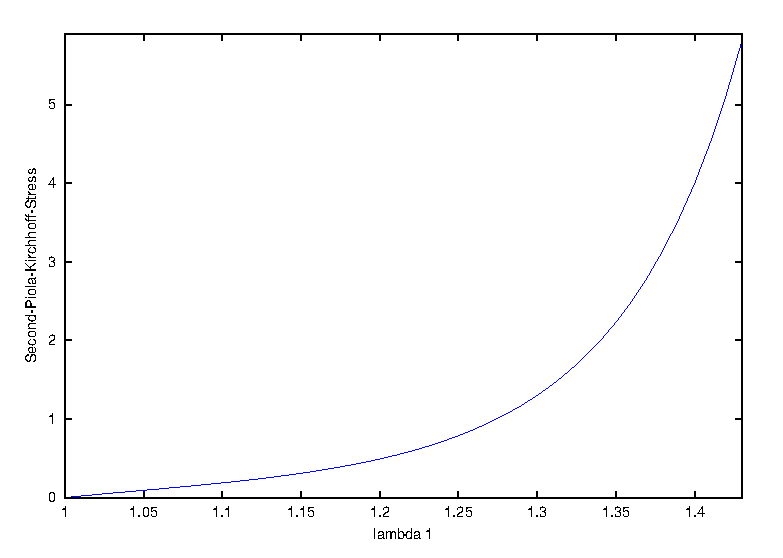
\includegraphics[width=80mm]{figures/stress-strain}
\end{center}

\subsubsection*{Parameters:}
\begin{tabular}{|c|c|c|}
	\hline
	Name inside Function	& Name to write in Inputfile	& Description \\ \hline \hline
	m		& M		& material parameter \\ \hline
	alpha		& APLPHA 	& material parameter\\ \hline
	beta		& BETA 		& material parameter \\ \hline
	gamma\_Pen	& GAMMA	 	& Parameter penalty function\\ \hline
	epsilon\_Pen	& EPSILON	 & Parameter penalty function\\ \hline
\end{tabular}

\subsubsection*{Line to describe itskov material in the input file:}
{\tt MAT 1 MAT\_ITSKOV  M 2.026255 ALPHA 20.0 BETA 20.0 EPSILON 100.0 GAMMA 100.0 DENS 1.0E-10}

\subsubsection*{Modified files:}
\begin{itemize}
	\item {\tt src/brick1/c1\_mat\_itskov.c}
	\par \noindent itskov material law 	
	\item {\tt src/brick1/brick1\_prototypes.h}
	\par \noindent declaration of the function {\tt c1\_mat\_itskov}	
	\item {\tt src/brick1/c1\_call\_mat.c}
	\par \noindent call of the function {\tt c1\_mat\_itskov}
	\par \noindent pass over densitiy
	\item {\tt src/input\_full/input\_material.c}
	\par \noindent definition of parameters from the input file
	\item {\tt src/headers/materials.h}
	\par \noindent definition of the structure {\tt ITSKOV} and insertion into the structure {\tt MATERIAL}
	\item {\tt src/headers/enums.h}
	\par \noindent insertion of {\tt m\_itskov} into the structure {\tt MATERIAL\_TYP}
\end{itemize}


\section{wallge}

Corresponding routine: wge\_call\_mat\\
`\cnl' is for line continuation.


\subsection{Isotropic gradient enhanced damage}

\cod{MAT\_Damage} \\ \\
\textbf{input:}
\begin{quote}
\begin{tabular}{ll}
\cod{MAT} $int$ \cnl & \\
\cod{YOUNG} $real$ \cnl& Young's modulus \\
\cod{NUE} $real$ \cnl& Poisson's ratio $\nu\in[0,0.5)$\\
\cod{Equival} $int$ \cnl& flag for equivalent strains \\
\cod{Damtyp} $int$ \cnl& flag for damage type \\
\cod{Kappa\_0} $real$ \cnl& initial damage equivalent strain \\
\cod{Kappa\_m} $real$ \cnl& factor for damage law \\
\cod{Alpha} $real$ \cnl& factor for exponential damage function \\
\cod{Beta} $real$ \cnl& factor for exponential damage function \\
\cod{k\_fac} $real$ & factor for de Vree 
\end{tabular} \\ \\
\end{quote}
\textbf{comment:} \\
\cod{Damtyp} has to be 2 (exponential damage), \cod{Equival} has to be 4 (equivalent strains 
based on de Vree, 1995). \\
No testfile available. \\
For more information, contact Andrea Hund.



\section{wall}

Corresponding routines: w1\_call\_mat, w1\_call\_matgeononl\\
`\cnl' is for line continuation.


\subsection{St. Venant Kirchhoff 2D}

\cod{MAT\_Struct\_StVenantKirchhoff} \\ \\
\textbf{input:}
\begin{quote} 
\begin{tabular}{ll}
\cod{MAT} $int$ \cnl & \\
\cod{YOUNG} $real$ \cnl& Young's modulus \\
\cod{NUE} $real$ \cnl& Poisson's ratio $\nu\in[0,0.5)$\\
\cod{DENS} $real$ \cnl& density $>0$\\
\cod{THEXPANS} $real$& thermal expansion coefficient
\end{tabular} \\ \\
\end{quote}
\textbf{example:}\\ 
\cod{MAT} 1 \cod{MAT\_Struct\_StVenantKirchhoff} \cod{YOUNG} 1000.0 \cod{NUE} 0.3 \cod{DENS} 0.001 
\cod{THEXPANS} 0.0078 \\ \\
\textbf{testfiles:}\\ 
Input/w1dyn.dat \\
Input/w1\_dyn\_dirich.dat \\
Input/w1\_Eulerstab.dat \\
Input/w1\_Eulerstab\_sd.dat \\
Input/w1\_gemm\_contact\_emconserv.dat \\
Input/w1\_neumann\_ortho.dat \\
Input/w1\_stalin\_dirich.dat \\
Input/tsi\_th2sta\_w1dyn\_3ele.dat\\ \\
\textbf{comment:}\\ 
Currently this is the only material for the wall element that is also implemented for the geometric 
nonlinear case and can be used in dynamic calculations.


\subsection{St. Venant Kirchhoff porous 2D}

\cod{MAT\_Struct\_STVENPOR} \\ \\
\textbf{input:}
\begin{quote} 
\begin{tabular}{ll}
\cod{MAT} $int$ \cnl & \\
\cod{YOUNG} $real$ \cnl& Young's modulus \\
\cod{NUE} $real$ \cnl& Poisson's ratio $\nu\in[0,0.5)$\\
\cod{DENS} $real$ \cnl& density $>0$\\
\cod{REFDENS} $real$ \cnl& reference density $>0$\\
\cod{EXPO} $real$ & exponent
\end{tabular} \\ \\
\end{quote}
\textbf{example:}\\ 
\cod{MAT} 1 \cod{MAT\_Struct\_STVENPOR} \cod{YOUNG} 21000000.0 \cod{NUE} 0.3 \cod{DENS} 0.3 
\cod{REFDENS} 1.0 \cod{EXPO} 2.5 \\ \\
\textbf{comment:}\\ 
For optimization problems. \\
Only for static, geometric linear calculations. \\
No testfile available.


\subsection{Von Mises material law 2D}

\cod{MAT\_MisesPlastic} \\ \\
\textbf{input:} 
\begin{quote}
\begin{tabular}{ll}
\cod{MAT} $int$ \cnl & \\
\cod{YOUNG} $real$ \cnl& Young's modulus \\
\cod{NUE} $real$ \cnl& Poisson's ratio $\nu\in[0,0.5)$\\
\cod{Sigy} $real$ \cnl& yield stress \\
\cod{BETAH} $real$ \cnl& controls the isotropic/kinematic hardening \\
\cod{Hard} $real$ \cnl& Hardening modulus (if hardening) \\
\cod{GF} $real$ \cnl& fracture energy (if softening) \\
(\cod{ALFAT} $real$ & temperature expansion factor)
\end{tabular} \\ \\
\end{quote}
\textbf{example:}\\ 
\cod{MAT} 1 \cod{MAT\_MisesPlastic} \cod{YOUNG} 10.0 \cod{NUE} 0.0 \cod{Xsi} 0.0 \cod{Sigy} 1.0 
\cod{Hard} 5.0 \\ \\
\textbf{testfiles:}\\ 
Input/w1\_mises.dat \\
Input/w1\_incompmode.dat \\ \\
\textbf{comment:}\\ 
Only for static, geometric linear calculations.\\
\cod{Xsi} (see example) is not read in. \\
Default value of \cod {BETAH}: $1.0$\\
\cod{ALFAT} can be read in (in src/input\_full/input\_material.c) but is not used anywhere.\\
Rotational symmetry is not implemented for plasticity $\to$ only plane strain and plane stress work.


\subsection{Von Mises material law 3D}

\cod{MAT\_3DMisesPlastic}\\ \\
\textbf{input:} 
\begin{quote}
\begin{tabular}{lcl}
\cod{MAT} $int$ \cnl & \\
\cod{YOUNG} $real$ \cnl& Young's modulus \\
\cod{NUE} $real$ \cnl& Poisson's ratio $\nu\in[0,0.5)$\\
\cod{Sigy} $real$ \cnl& yield stress \\
\cod{BETAH} $real$ \cnl& controls the isotropic/kinematic hardening \\
\cod{Hard} $real$ \cnl& Hardening modulus (if hardening) \\
\cod{GF} $real$ \cnl& fracture energy (if softening) \\
(\cod{ALFAT} $real$ & temperature expansion factor)
\end{tabular} \\ \\
\end{quote}
\textbf{example:}\\ 
\cod{MAT} 1 \cod{MAT\_3DMisesPlastic} \cod{YOUNG} 25850.0 \cod{NUE} 0.18 \cod{Xsi} 0.0 \cod{Sigy} 1.9 
\cod{GF} 0.06 \\ \\
\textbf{testfile:}\\ 
Input/w1\_3DmisGF.dat \\ \\
\textbf{comment:}\\ 
Only for static, geometric linear calculations.\\
Default value of \cod{BETAH}: $1.0$\\
\cod{ALFAT} can be read in (in src/input\_full/input\_material.c) but is not used anywhere.\\
Rotational symmetry is not implemented for plasticity $\to$ only plane strain and plane stress work.\\
Links to src/materials/mat\_pl\_mises\_lin.c ($\to$ global material, see \ref{global_mises}).


\subsection{Drucker-Prager material law 2D}

\cod{MAT\_DP\_Plastic} \\ \\
\textbf{input:} 
\begin{quote}
\begin{tabular}{ll}
\cod{MAT} $int$ \cnl & \\
\cod{YOUNG} $real$ \cnl& Young's modulus \\
\cod{NUE} $real$ \cnl& Poisson's ratio $\nu\in[0,0.5)$\\
(\cod{ALFAT} $real$ \cnl& temperature expansion factor)\\
\cod{Sigy} $real$ \cnl& yield stress \\
\cod{PHI} $real$ \cnl& angle of friction\\
\cod{Hard} $real$ \cnl& Hardening modulus (if hardening) \\
(\cod{GF} $real$ \cnl& fracture energy (if softening) ) \\
(\cod{BETAH} $real$ & controls the isotropic/kinematic hardening)
\end{tabular} \\ \\
\end{quote}
\textbf{example:}\\ 
\cod{MAT} 1 \cod{MAT\_DP\_Plastic} \cod{YOUNG} 30e3 \cod{NUE} 0.0 \cod{Sigy} 2.0 \cod{BETAH} 0.0 \cod{Hard}
-0.3 \cod{PHI} 40.0 \\ \\
\textbf{comment:}\\ 
Only for static, geometric linear calculations.\\
Fracture energy can be read in (in src/input\_full/input\_material.c) but is not used $\to$ implementation 
only for hardening.\\
The value read in for \cod{BETAH} is not used, instead the default value of $1.0$ is applied.\\
\cod{ALFAT} can be read in (in src/input\_full/input\_material.c) but is not used anywhere.\\
Rotational symmetry is not implemented for plasticity (even though headline of material routine tells so) 
$\to$ only plane strain and plane stress work. \\
No testfile available.


\subsection{Elastoplastic concrete material law 2D}

\cod{MAT\_ConcretePlastic} \\ \\
\textbf{input:}
\begin{quote} 
\begin{tabular}{ll}
\cod{MAT} $int$ \cnl & \\
\end{tabular}
\end{quote}
input for concrete
\begin{quote}
\begin{tabular}{ll}
\cod{YOUNG} $real$ \cnl& Young's modulus \\
\cod{NUE} $real$ \cnl& Poisson's ratio $\nu\in[0,0.5)$\\
(\cod{DENS} $real$ \cnl& density $>0$)\\
(\cod{ALFAT} $real$ \cnl& temperature expansion factor) \\
(\cod{XSI} $real$ \cnl)&\\
(\cod{Sigy} $real$ & yield stress) \\
\textit{new line in inputfile}& \\
\cod{FTM} $real$ \cnl& tensile strength \\
\cod{FCM} $real$ \cnl& compressive strength \\
\cod{GT} $real$ \cnl& tensile fracture energy \\
\cod{GC0} $real$ \cnl& compressive fracture energy \\
\cod{GAMMA1} $real$ \cnl&\\
\cod{GAMMA2} $real$ \cnl&\\
\end{tabular}
\end{quote}
input for tension stiffening
\begin{quote}
\begin{tabular}{ll}
\cod{NSTIFF} $real$ &\\
\end{tabular}
\end{quote}
input for rebars 
\begin{quote}
\begin{tabular}{ll}
\textit{new line in inputfile}& \\
\cod{MAXREB} $real$ & number of rebars\\
\textit{new line in inputfile}& \\
(\cod{REBAR} $real$ \cnl) &\\
\cod{REBAREA} $real$ \cnl& rebar area \\
\cod{REBANGLE} $real$ \cnl& rebar angle\\
\cod{REBSO} $real$ \cnl&\\
\cod{REBDS} $real$ \cnl&\\
\cod{REBGAMMA} $real$ &\\
\textit{new line in inputfile}& \\
(\cod{REBDENS} $real$ \cnl& rebar density $>0$) \\
(\cod{REBALFAT} $real$ \cnl& rebar temperature expansion factor)\\
(\cod{REBEMOD} $real$ \cnl& rebar Young's modulus)\\
(\cod{REBNUE} $real$ & rebar Poisson's ratio $\nu\in[0,0.5)$)\\
\textit{new line in inputfile}& \\
(\cod{REBSIGY} $real$ \cnl& rebar yield stress)\\
(\cod{REBHARD} $real$ & rebar hardening modulus)\\
\textit{new line in inputfile}& \\
... & additional rebar data if \cod{MAXREB} $>0$ 
\end{tabular} \\ \\
\end{quote}
\textbf{comment:}\\ 
Concrete + rebars.\\
Only for static, geometric linear calculations.\\
All parameters in parentheses can be read in (in src/input\_full/input\_material.c) but are not used.\\
Default values of \cod{GAMMA1} and \cod{GAMMA2}: $3.0$ and $\frac{6.0}{5.0}$, respectively.\\
If \cod{GAMMA1} is chosen to be $<1.0$, then \cod{GAMMA1} is set to $3.0$.\\
Rotational symmetry is not implemented for plasticity $\to$ only plane strain and plane stress work.\\
No testfile available.\\
For more information, contact Andrea Hund.


\subsection{Elastoplastic concrete material law 3D}

\cod{MAT\_3DConcretePlastic} \\ \\
\textbf{input:} 
\begin{quote}
\begin{tabular}{ll}
\cod{MAT} $int$ \cnl & \\
\cod{YOUNG} $real$ \cnl& Young's modulus \\
\cod{NUE} $real$ \cnl& Poisson's ratio $\nu\in[0,0.5)$\\
\cod{FTM} $real$ \cnl& tensile strength \\
\cod{FCM} $real$ \cnl& compressive strength \\
\cod{GT} $real$ \cnl& tensile fracture energy \\
\cod{GC} $real$ \cnl& compressive fracture energy \\
(\cod{DFAC} $real$ \cnl& damage factor: $0.0$ plastic - $1.0$ fully damaged)\\
\cod{GAMMA1} $real$ \cnl& fitting parameter yield function $1$\\
\cod{GAMMA2} $real$ \cnl& symm. biaxial compression stressfactor\\
\cod{GAMMA3} $real$ \cnl& fitting parameter to account for HPC $\to$ Haufe ($=\frac{1}{3}$ for normal concrete)\\
\cod{GAMMA4} $real$ & fitting parameter to account for HPC $\to$ Haufe ($=\frac{4}{3}$ for normal concrete)
\end{tabular} \\ \\
\end{quote}
\textbf{example:}\\ 
\cod{MAT} 1 \cod{MAT\_3DConcretePlastic} \cod{YOUNG} 30000.0 \cod{NUE} 0.2 \cod{FTM} 3.0 \cod{FCM} 40.0 
\cod{GT} 0.12 \cod{GC} 50.0 \\ \\
\textbf{testfile:}\\ 
Input/w1\_epc3D.dat \\ \\
\textbf{comment:}\\ 
Only concrete, no rebars.\\
Only for static, geometric linear calculations.\\
The same 3D formulation as used for multilayer materials ($\to$ see thesis of Menrath and Haufe).\\
An unsymmetric solver should be used if trial stresses could be in the apex region (general warning print out is done).\\
Default values: \cod{DFAC}$=0.5$, \cod{GAMMA1}$=3.0$, \cod{GAMMA2}$=\frac{6.0}{5.0}$, \cod{GAMMA3}$=\frac{1.0}{3.0}$, 
\cod{GAMMA4}$=\frac{4.0}{3.0}$.\\
\cod{DFAC} can be read in (in src/input\_full/input\_material.c) but is not used.\\
Rotational symmetry is not implemented for plasticity $\to$ only plane strain and plane stress work.\\
Links to src/materials/mat\_pl\_epc\_main.c ($\to$ global material, see \ref{global_concrete}).


\subsection{Isotropic 2D damage model}

\cod{MAT\_DAM\_MP} \\ \\
\textbf{input:} 
\begin {quote}
\begin{tabular}{ll}
\cod{MAT} $int$ \cnl & \\
\cod{YOUNG} $real$ \cnl& Young's modulus \\
\cod{NUE} $real$ \cnl& Poisson's ratio $\nu\in[0,0.5)$\\
\cod{KAPPA\_0} $real$ \cnl& initial damage equivalent strain (guess) \\
\cod{ALPHA} $real$ \cnl& factor for exponential damage function(guess)\\
\cod{BETA} $real$ & factor for exponential damage function (guess)
\end{tabular} \\ \\
\end{quote}
\textbf{example:}\\ 
\cod{MAT} 1 \cod{MAT\_DAM\_MP} \cod{YOUNG} 7350000.0 \cod{NUE} 0.18 \cod{KAPPA\_0} 5.0 \cod{ALPHA} 0.99 \cod{BETA} 10.0 \\ \\
\textbf{comment:}\\ 
Only for static, geometric linear calculations.\\
Applies to interface element according to documentation.\\
Damage model of Mazars/Pijaudier-Cabot $\to$ PDH-Peerlings.\\
Implementation only for plane stress.\\
No testfile available.


\subsection{Linear elastic 2D damage model}

\cod{MAT\_Damage} \\ \\
\textbf{input:} 
\begin{quote}
\begin{tabular}{ll}
\cod{MAT} $int$ \cnl & \\
\cod{YOUNG} $real$ \cnl& Young's modulus \\
\cod{NUE} $real$ \cnl& Poisson's ratio $\nu\in[0,0.5)$\\
\cod{Equival} $int$ \cnl& flag for equivalent strains\\
\cod{Damtyp} $int$ \cnl& flag for damage type\\
\cod{Kappa\_0} $real$ \cnl& initial damage equivalent strain \\
\cod{Kappa\_m} $real$ \cnl& factor for damage law\\
\cod{Alpha} $real$ \cnl& factor for exponential damage function\\
\cod{Beta} $real$ \cnl& factor for exponential damage function\\
\cod{k\_fac} $real$ & factor for de Vree
\end{tabular} \\ \\
\end{quote}
\textbf{example:}\\ 
\cod{MAT} 1 \cod{MAT\_Damage} \cod{YOUNG} 7350000.0 \cod{NUE} 0.18 \cod{Equival} 4 \cod{Damtyp} 2 \cod{Kappa\_0} 5.0 
\cod{Kappa\_m} 10.0 \cod{Alpha} 0.99 \cod{Beta} 10.0 \cod{k\_fac} 1.0\\ \\
\textbf{testfile:}\\
Input/struct2ml\_ifvers.dat \\ \\
\textbf{comment:}\\ 
Only for static, geometric linear calculations.\\
\cod{Equival}$=1$ energy release rate concept - thermodynamics\\
\cod{Equival}$=2$ Simo \& Ju (1987)\\
\cod{Equival}$=3$ Ju (1989)\\
\cod{Equival}$=4$ de Vree (1995)\\
\cod{Damtyp}$=1$ linear softening damage\\
\cod{Damtyp}$=2$ exponential damage\\
Implementation only for rotational symmetry.\\



\section{Suggestions}
\begin{enumerate}
\item Problem with commented input file, comments break CCarat input ---
  fixed.
\item Expand unified material description to all elements, see e-mail
  underneath 
\item Materials in the new discretization
\end{enumerate}